\section{Results}

\begin{figure}[htb]
    \centering
    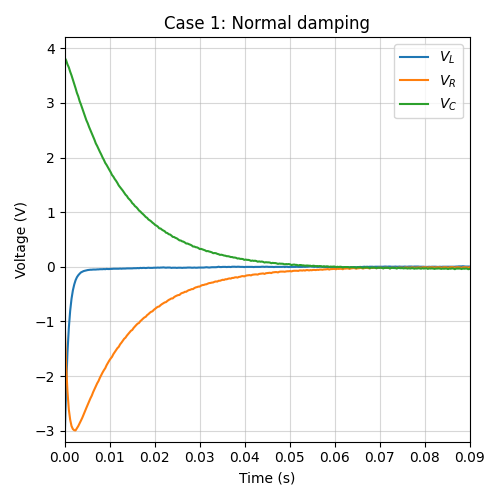
\includegraphics[width=\linewidth]{fig/case1_normal_damping}
    \caption{Signals showing normal damping behaviour.}\label{fig:normal_damp}
\end{figure}

In Figure~\ref{fig:normal_damp}, the circuit is normally damped such that the components discharge gradually over
the cycle to zero volts without oscillating.
The resistance value chosen here was calculated using double the critical system resistance found in Eq.~\eqref{eq:crit_damp}, which ended up being \qty{1133}{\ohm}.

\begin{figure}[htb]
    \centering
    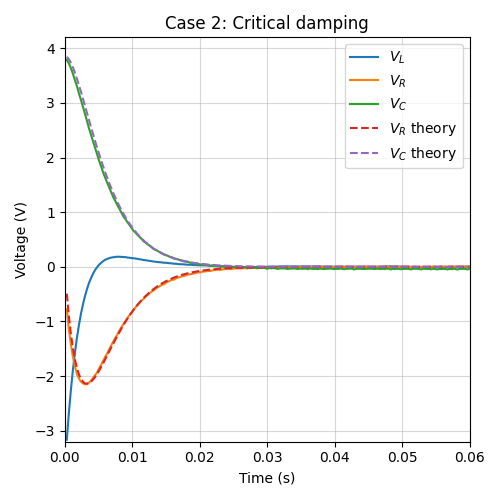
\includegraphics[width=\linewidth]{fig/case2_crit_damping}
    \caption{Signals showing critical damping behaviour.}\label{fig:crit_damp}
\end{figure}

In Figure~\ref{fig:crit_damp}, the resistance chosen using Eq.~\eqref{eq:crit_damp} was \qty{485}{\ohm}.
Notice the quicker time to reach zero volts compared with case 1.

\begin{figure}[htb]
    \centering
    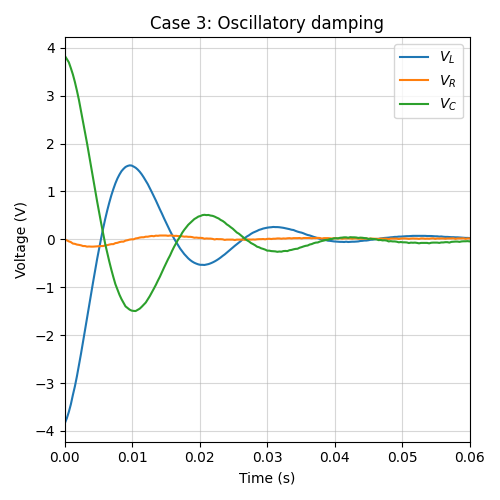
\includegraphics[width=\linewidth]{fig/case3_oscillatory_damping}
    \caption{Signals showing oscillatory damping.}\label{fig:osc_damp}
\end{figure}

Figure~\ref{fig:osc_damp} shows that at selected resistance \qty{20}{\ohm}, the behaviour turned oscillatory.
Since the resistance was much lower, more of the electric potential remained within the inductor and capacitor during
the whole discharge cycle.

\begin{figure}[htb]
    \centering
    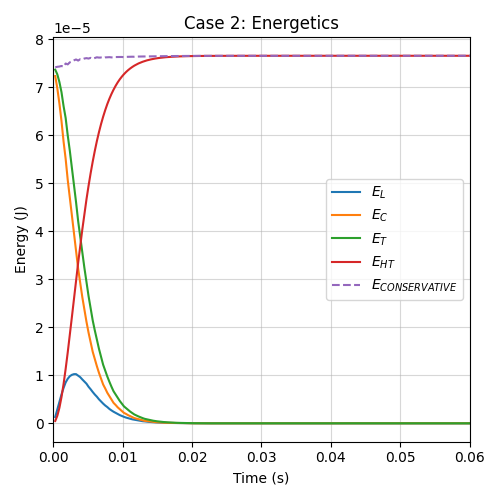
\includegraphics[width=\linewidth]{fig/case2_energetics}
    \caption{Critically damped energetics}\label{fig:case2_energy}
\end{figure}

\begin{figure}[htb]
    \centering
    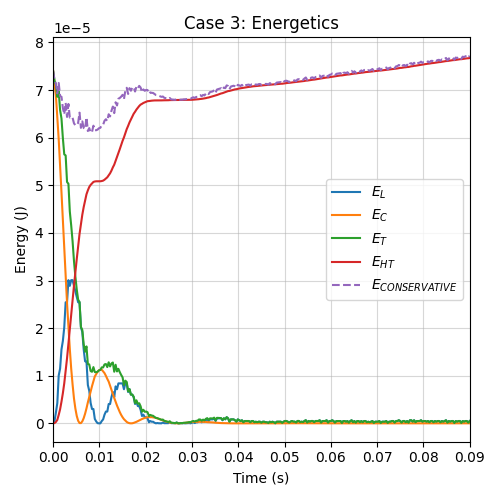
\includegraphics[width=\linewidth]{fig/case3_energetics}
    \caption{Oscillatory energetics}\label{fig:case3_energy}
\end{figure}

Figures~\ref{fig:case2_energy} and~\ref{fig:case3_energy} demonstrate the energetics of the system in critically
damped and oscillatory cases.
In both figures, it shows that once the discharge is initiated, the stored energy transfers between the
electric and magnetic fields of the circuit.
As $E_T$ decreases, the accumulated dissipated thermal energy, $E_{HT}$,
rises due
to joule heating.

\begin{table}[htbp]
    \caption{Oscillation Frequency}
    \begin{tabular}{lrrl}
        \toprule
        {Quantity}                      & {Value}           & {Units} \\
        \midrule
        Experimental frequency          & 46                & Hz      \\
        Theoretical natural frequency   & \qty{49.1(1.8)}{} & Hz      \\
        Theoretical frequency incl. $R$ & \qty{47.1(1.6)}{} & Hz      \\
        \bottomrule
    \end{tabular}\label{tab:osc_freq}
\end{table}

The oscillation frequency results are listed in Table~\ref{tab:osc_freq}.
Experimental frequency was determined by measuring the peak-peak time and dividing by the period.
Theoretical values were calculated using Eq.~\eqref{eq:freq}.
The theoretical natural frequency is close, but not quite consistent with the determined value, however, the
theoretical frequency taking into account $R$ is consistent.
This suggests the small damping resistance produces a system frequency lower than the natural frequency.
Note: Uncertainties in values were calculated using the aid of the \textit{uncertainties} python package.


